\documentclass[11pt]{article}

\usepackage{deauthor}
\usepackage{times,graphicx}

% user packages
\usepackage{todonotes}
\usepackage{pifont}
\newcommand{\cmark}{\ding{51}}
\newcommand{\xmark}{\ding{55}}
\usepackage{multirow}
\usepackage{booktabs}
\usepackage{graphicx}

\title{Logical Queries on Knowledge Graphs: \\ Emerging Interface of Incomplete
Relational Data}

\author{Zihao Wang$^{\dagger}$
\hspace{2em} Hang Yin$^{\ddagger}$
\hspace{2em} Yangqiu Song$^{\dagger}$ \\
$^{\dagger}$ Department of CSE, HKUST, Hong Kong, China \hspace{1em}
\texttt{\small\{zwanggc,yqsong\}@cse.ust.hk}\\
$^{\ddagger}$ Tsinghua University, Beijing, China \hspace{1em} \texttt{\small h-yin20@mails.tsinghua.edu.cn}}

% unnecessary commands
\usepackage{paralist}
\newcommand{\entity}{\mathcal{E}}
\newcommand{\relation}{\mathcal{R}}
\newcommand{\lang}{\mathcal{L}}
\newcommand{\model}{\mathcal{M}}
\newcommand{\term}{\mathcal{T}}
\newcommand{\kgnew}{\mathcal{KG}}

\begin{document}

\maketitle
\begin{abstract}
As a graph abstraction of real-world relational data, knowledge graphs contain large amounts of factual knowledge but suffer from incompleteness. Such incompleteness, also known as the open-world assumption, prevents logical queries from being answered through the query-answering paradigms for relational databases. In this paper, we discuss how learning-based models bridge incomplete relational data and logical queries from the perspective of rigorous formal logic. Existing works are structured as a three-party game among knowledge graphs, logical queries, and learning-based models. Compared to the well-established tale between databases and queries in the database theory, current achievements are still preliminary. Our work pointed out several possible directions for future work.
\end{abstract}

\section{Introduction}
The knowledge graph is perhaps one of the simplest representations of relational knowledge~\cite{Bollacker2008Freebasecollaboratively,Vrandecic2014Wikidatafree,PellissierTanon2016FreebaseWikidata}. A knowledge graph contains a large number of triples, where each triple $(h, r, t)$ contains a head entity $h$, a tail entity $t$, and the relation $r$ in between. Such a simple format enables factual knowledge to be adapted to answer real-world questions~\cite{Sun2022JointLKJoint,Yasunaga2021QAGNNReasoning,Saxena2021QuestionAnswering,Ren2021LEGOLatent,Lin2019KagNetKnowledgeAware}.

Under the view of data engineering, a knowledge graph is no more than a (relational) database~\cite{abiteboul1995FoundationsDatabases}. It is natural to expect first-order queries, a fundamental type of relational database queries that have been well-understood theoretically~\cite{Libkin2004ElementsFinite} and efficiently solved practically~\cite{Kroenke2018Databaseprocessing}, can also be answered on knowledge graphs. However, applying the existing query-answering algorithms designed for (relational) databases can not address logical queries on knowledge graphs.
The major obstacle is that large-scale knowledge graphs are inherently incomplete. Modern large-scale knowledge graphs are constructed by crowd-sourcing~\cite{Vrandecic2014Wikidatafree} or even by automatic information extraction pipelines~\cite{Carlson2010ArchitectureNeverEnding}.  Given an observed knowledge graph, the non-existence of a triple does not imply that such a triple is not part of the underlying knowledge graph. This issue is acknowledged as the open-world assumption~\cite{Libkin2009OpenClosed}.
Therefore, the actual answers to logical queries are not guaranteed by running existing query-answering algorithms on knowledge graphs.

The issue of missing knowledge founds its partial solution with learning-based models.
Models that learn from the existing observed triples can predict the missing triples in the underlying knowledge graph. The research topic focusing on the prediction of missing triples with learned embeddings is known as knowledge graph representation or knowledge base completion~\cite{Ji2022Surveyknowledge,Ruffinelli2020YouCAN}.
Then, the logical queries can be addressed by combining the query-answering algorithms and the learning-based models~\cite{Ren2020Query2boxReasoning,Kotnis2021AnsweringComplex,Daza2020MessagePassing}.
The participation of learning-based models brings unique strengths and weaknesses to logical query answering, especially compared to traditional query answering algorithms for relational databases~\cite{Ren2020Query2boxReasoning}. For traditional databases, query-answering algorithms are discussed from the data perspective and the query perspective. The complexity of such algorithms is characterized by the data complexity (the complexity grows with the size of the database) and the query complexity (the complexity grows with the size of the query), respectively.
When answering logical queries with learning-based models, it is essential to understand how learning-based models interact with knowledge graphs (model-data interaction) and logical queries (model-query interaction), besides how to design, train, and infer such models.

In this paper, we review recent advancements in logical query answering on knowledge graphs. Our introduction begins with how to define the problems and construct datasets and then to learning-based query answering methods. Our discussion is organized from three perspectives: knowledge graphs (data) perspective, logical query perspective, and model perspective.
Section~\ref{sec:data-query} introduces the logical query answering tasks on knowledge graphs in the rigorous language of model theory. All existing datasets and benchmarks are discussed in Section~\ref{sec:dataset} based on the rigorous definitions.
Section~\ref{sec:method} discusses the learning-based methods for knowledge graph logical query answering. Existing approaches are categorized by their interaction with the knowledge graph (data perspective) and the logical queries (query perspective).
Section~\ref{sec:future} discusses the limitation of the existing work and several possible future directions.

\section{Preliminaries for Logical Queries}\label{sec:data-query}
Logical queries are formally defined by $\lang$-formula on an $\lang$-structure, which are central concepts in model theory~\cite{Marker2002Modeltheory}. Specifically, $\lang$-structure rigorously justifies the concept of knowledge graphs while $\lang$-formula formally defines the scope of queries. Formal definitions provide a framework to investigate the data and the query aspects of the knowledge graph logical query answering tasks.

The minimal and informal description of knowledge graphs is a set of triples $\{(h_i, r_i, t_i)\}$ that encapsulates the real-world knowledge, where $h_i, t_i\in \entity$ are the head and tail entities and $r_i\in \relation$ is the connected relation. Formally speaking, a knowledge graph is an $\lang_{KG}$-structure defined by a language $\lang_{KG}$ for knowledge graphs. The concept of language and structure, which concerns syntax and semantics of first-order logic respectively, is defined in Definition~\ref{def:language} and Definition~\ref{def:structure}.

\begin{definition}[Language]~\label{def:language}
    A language $\lang$ is a triple $(\entity, \relation, \mathcal{F})$ where $\entity$ is the set of constant symbols, $\relation$ is the set of predicate symbols, and $\mathcal{F}$ is the set of function symbols. For each $r\in \relation$ and $f\in \mathcal{F}$, associated integers $n_r$ and $n_f$ indicate the number of inputs for $R$ and $F$, respectively.
\end{definition}
All (classic) knowledge graphs can be described by a language $\lang_{KG}$ by letting (1) $\relation$ be the set of binary relations ($n_r=2$), (2) the constant set $\entity$ is finite and contains all entities, and (3) $\mathcal{F} = \emptyset$. $\entity$ and $\relation$ are finite sets without further classification.


\begin{definition}[$\lang$-structure]~\label{def:structure}
    An $\lang$-structure $\model$ for the language $\lang$ is a pair $(M,I)$,where M is a non-empty set called the universe of $\model$ and $I$ is an interpretation function that:
    (i) For each $c\in \entity, I(C)\in M$;
    (ii)  For each $r\in \relation, I(r) \subset M^{n_r}$ , where $n_r$ is the size of relations;
    (iii) For each $f\in \mathcal{F}$, a function $I(f): M^{n_f}\mapsto M$ , where $n_f$ is the number of inputs in $f$.
\end{definition}

A knowledge graph  $\kgnew$ induces an $\lang_{KG}$-structure by letting $M = \entity$ (with $\forall e\in \entity, I(e) = e$), so that each relation $I(r)$ is a subset of $M^2$.
The open world assumption of knowledge graphs can then be formally stated in Definition~\ref{def:owa}.
\begin{definition}[Open world assumption]\label{def:owa}
For a given language $\lang_{KG}$ of knowledge graph, there is an \textbf{u}nderlying $\lang_{KG}$-structure $\kgnew_u$, and one (or more) \textbf{o}bserved $\lang_{KG}$-structure (s) $\kgnew_o$, such that for each relation $r\in \relation$, the relation set of $\kgnew_o$ and $\kgnew_u$ satisfies $I_{\kgnew_o}(r) \subseteq I_{\kgnew_u}(r) \subseteq M^2$.
\end{definition}

Then, it is ready to define the logical queries with formal concepts, including $\lang$-terms and $\lang$-formulae.
The current discussion focuses on first-order logic.
\begin{definition}[$\lang$-term]\label{def:term}
$\lang$-terms be the smallest set of $\term$ such that:
(i) $e\in\term$ for each constant symbol $e \in \entity$;
(ii) Any variable $v_i \in \term$ for 1, 2, ... ;
(iii) if $t_1, t_2, ..., t_{n_f}\in \term$ and $f \in \mathcal{F}$, then $f(t_1, ..., t_{n_f}) \in \term$.
\end{definition}
\begin{definition}[Atomic $\lang$-formula]\label{def:atomic-formula}
    $\phi$ is an atomic $\lang$-formula if $\phi$ is $r(t_1, ..., t_{n_r})$, where $r\in \relation$ is a relation symbol and $t_\cdot$ are $\lang$-terms. Given $\lang$-structure $\model$ , we say $\model\models r(r_1, ..., r_{n_r})$ is True if and only if the tuple $(t_1, ..., t_{n_r})\in I(r)$.
\end{definition}
\begin{definition}[$\lang$-formula]\label{def:formula}
The set of $\lang$-formula is the smallest set $\Phi$ containing all atomic formulae such that: (i) if $\phi \in \Phi$, then $\lnot \phi \in \Phi$; (ii) if $\phi, \psi\in \Phi$, then $(\phi\land \psi) \in \Phi$ and $(\phi \lor \psi)\in \Phi$; (iii) if $\phi \in \Phi$ and $v_i$ is any variable, then $\exists v_i \phi \in \Phi$ and $\forall v_i \phi \in \Phi$.
\end{definition}
We say a variable $v$ is \textit{free} if there are no associated quantifiers. Otherwise, it is \textit{bounded}. We use $\phi(v)$ indicates the $\lang$-formula $\phi$ contains a free variable $v$. An $\lang$-formula without free variables is called an $\lang$-sentence. Logical queries are $\lang$-formulae and can be evaluated given a knowledge graph $\kgnew$.
As studied in the database literature~\cite{VandenBroeck2017QueryProcessing}, we discuss boolean queries, set-valued queries, and aggregate queries.

\noindent A \textbf{boolean query} is an $\lang_{KG}$-sentence $s$. Given the $\lang_{KG}$-structure $\model$, its answer is the boolean value indicating whether $\model \models s$ or not.

\noindent A \textbf{set-valued query} is an $\lang_{KG}$-formula $\phi$ with exactly one free variable $v$. Given  the $\lang$-model $\model$, its answer set is $\{e:  e\in \entity, \model\models \phi(v=e) \}$.

\noindent An \textbf{aggregate query} looks for the aggregation statistics of the answer set of a set-valued query, such as counting, summation, and so on.


\section{Logical Query Answering Datasets and Evaluations}\label{sec:dataset}
Based on the formal concepts given in Section~\ref{sec:data-query}, we are ready to formally justify existing datasets from the knowledge graphs (the data perspective) that are queried and the scope of logical queries (the query perspective) to be answered. Instead of going through all existing datasets, we discuss the underlying knowledge graphs and logical queries.

\begin{table}[t]
%	\small
	\centering
	\caption{Summation of open source knowledge graphs used in the existing datasets. KGs are sorted by the number of entities.}~\label{tab:knowledge-graphs}
	\begin{tabular}{lrrrrr}
		\toprule
		Knowledge graph & \# Entities & \# Relations & \# Total edges & Comment & Datasets \\
		\midrule
%		FB15k-237-v3~\cite{teru2020InductiveRelationPrediction} & 4,000 / 3,000 & 218 / 187 & 22,394 / 9,137 & Train graph /Inductive test graph & \cite{hu2022TypeawareEmbeddingsMultiHopa}\\
%		NELL955-v3~\cite{teru2020InductiveRelationPrediction} & 4,674 / 4,921 & 142 / 122 & 20,117 / 9,668 & Train graph / Inductive test graph & \cite{hu2022TypeawareEmbeddingsMultiHopa}\\
		FB15k-237~\cite{Bordes2013TranslatingEmbeddings} & 14,505 & 237 & 310,079 & - & \cite{Ren2020Query2boxReasoning,Ren2020BetaEmbeddings,Galkin2022InductiveLogical,Hu2022TypeawareEmbeddings,Wang2021BenchmarkingCombinatorial}\\
		FB15k~\cite{Toutanova2015Observedlatent} & 14,951 & 1,345 & 592,213 & - & \cite{Ren2020Query2boxReasoning,Ren2020BetaEmbeddings,Wang2021BenchmarkingCombinatorial}\\
		DBPedia~\cite{Auer2007DBpediaNucleus} & 34,575 & 3 & 240,942 & Hierarchical KG & \cite{Choudhary2021SelfSupervisedHyperboloidc} \\
		WN18RR~\cite{Miller1995WordNetlexical} & 40,903 & 11 & 103,509 & Hierarchical KG & \cite{Huang2022LinELogical}\\
		NELL955~\cite{xiong2017deeppath} & 63,361 & 200 & 142,804 & - & \cite{Ren2020Query2boxReasoning,Ren2020BetaEmbeddings,Hu2022TypeawareEmbeddings,Wang2021BenchmarkingCombinatorial}\\
		% WD50K~\cite{Galkin2020MessagePassing} & 47,156 & 532 & 236,507 & Hyperrelational KG & \cite{Alivanistos2022QueryEmbedding} \\
		DRKG~\cite{Zhang2021Drugrepurposing} & 97,238 & 107 & 5,874,271 & - & \cite{Choudhary2021ProbabilisticEntity} \\
		% E-commerce & about 118,000 & 4 & about 562,000 & Not released & \cite{Choudhary2021SelfSupervisedHyperboloidc} \\		
        FB400k~\cite{Talmor2018WebKnowledgeBase,Bollacker2008Freebasecollaboratively} & 409,829 & 918 & 2,151,671 & - & \cite{Ren2022SMOREKnowledgea} \\
		ogbl-wikikg2~\cite{Hu2020OpenGraph} & 2,500,604 & 535 & 17,137,181 & - & \cite{Ren2022SMOREKnowledgea,Galkin2022InductiveLogical} \\
		Freebase~\cite{Bollacker2008Freebasecollaboratively} & 86,054,151 & 14,824 & 338,586,276 & - & \cite{Ren2022SMOREKnowledgea} \\
		\bottomrule
	\end{tabular}
\end{table}

\subsection{Knowledge Graphs} Table~\ref{tab:knowledge-graphs} shows the knowledge graphs investigated in existing datasets. Existing evaluation includes knowledge graphs of different scales (from $10^3$ to $10^9$) and various properties. Notably, the knowledge graphs with hierarchical relation~\cite{Miller1995WordNetlexical,Auer2007DBpediaNucleus} contain the prior and more complicated structures on entities and relations, respectively, which could be leveraged to improve the performance of query answering method.
Inductive logical query answering~\cite{Galkin2022InductiveLogical} also considers an inductive
KG setting~\cite{Teru2020InductiveRelation}, which is more challenging under the open-world assumption.

\subsection{Logical Queries} The scope of queries that can be answered is not rigorously justified in the existing works. Though some works claim they are addressing the first-order queries~\cite{Ren2020BetaEmbeddings} or logical queries in general~\cite{Liu2021NeuralAnsweringLogical}, their definitions are still a strict subset of the first-order queries defined in Definition~\ref{def:formula}.
Table~\ref{tab:query-families} summarizes the formal definitions for three typical query families. The scopes of three query families are sorted in increasing order, i.e., CQ $\subseteq$ EPFO $\subseteq$ EFO. The universal quantifier $\forall$ is not widely discussed because its semantics is not usually interpretable over the knowledge graphs. This is the same order for query families that learning-based query answering methods tried to solve.


\begin{table}[t]
	\centering
	\caption{Formal definitions of three typical query families. Compared to the first-order logic formula defined formally with Definition~\ref{def:formula}, three query families are defined using a subset of connectives or quantifiers (indicated by \cmark).}\label{tab:query-families}
	\begin{tabular}{lccccc}
		\toprule
		Query Family & $\land$ & $\lor$ & $\lnot$ & $\exists$ & $\forall$ \\\midrule
		Conjunctive Query (CQ) & \cmark & \xmark & \xmark & \cmark & \xmark \\
		Existential Positive First Order (EPFO) & \cmark & \cmark & \xmark & \cmark & \xmark \\
		Existential First Order (EFO) & \cmark & \cmark & \cmark & \cmark & \xmark \\
        % \midrule
        % First Order (FO, with Definition~\ref{def:formula}) & \cmark & \cmark & \cmark & \cmark & \cmark \\
		\bottomrule
	\end{tabular}
\end{table}

However, additional assumptions are made so that queries are more suitable to be answered by learning-based methods. Common assumptions include that (1) the query is assumed to be acyclic and (2) only one free variable in the logical formula. The first assumption skips the queries that may involve hard constraint satisfaction problems and the second assumption restricts the space complexity of search within $O(|\entity|)$. These assumptions are not necessary for all learning-based models. For example, BiQE~\cite{Kotnis2021AnsweringComplex} accepts conjunctive queries with multiple free variables, and CQD~\cite{Arakelyan2021ComplexQuery} answers general EPFO queries without any additional assumptions.
Most existing datasets are usually constructed as companions to evaluate the proposed methods, especially query embedding methods with the operator tree representation discussed in Section~\ref{sec:qe-optree}. Such methods assume the answers with respect to the only free variable can be computed by executing learnable set operators. The execution order of set operators is decided by compiling the query formula into an operator tree.
Thus, popular datasets~\cite{Ren2020Query2boxReasoning,Ren2020BetaEmbeddings,Wang2021BenchmarkingCombinatorial} for EPFO and EFO queries also accept implicit assumptions:
(1) the only free variable $v$ is assumed to be the root of the set operator tree;
(2) all leaf nodes must be constant entity symbols rather than existential variables.

We see that these assumptions are not related to the logic but only to make the queries easier to solve by a special class of learning-based methods. There are no serious empirical evaluations for queries without such assumptions.

\subsection{Evaluation Metrics}
The query families are categorized by the formulation of logical formulae. Moreover, for each family, it is also able to construct three types of queries. Here we list popular evaluating metrics.
\begin{itemize}
\item For \textbf{boolean query}, this becomes a classification problem, and thus standard classification metrics can be applied, like ROC AUC score~\cite{Ren2020BetaEmbeddings, Hamilton2018EmbeddingLogical}.
\item For \textbf{set-valued query}, standard metrics include Mean Reciprocal Rank (MRR)~\cite{Ren2020Query2boxReasoning},  Adjusted Mean Rank Index (AMRI)~\cite{Alivanistos2022QueryEmbedding}, Average percentile rank (APR)~\cite{Hamilton2018EmbeddingLogical}, and Hits at K (H@K)~\cite{Ren2020Query2boxReasoning}.
\item For \textbf{aggregate query}, counting is the only problem that has been considered. Spearman's rank correlation coefficient~\cite{Ren2020BetaEmbeddings} and Pearson's correlation coefficient~\cite{Luus2021LogicEmbeddings} have been proposed when the model is incapable of predicting the precise number. Otherwise, Mean Absolute Error (MAE) is used~\cite{Luus2021LogicEmbeddings}.
\end{itemize}

\section{Learning-Based Methods}\label{sec:method}
Traditional database query answering algorithms are executed over the raw data to find the answers, see Figure~\ref{subfig:dbqa}. This paradigm fails in the cases of knowledge graph queries, where the underlying data is not observed.
Current knowledge graph logical query answering methods address the open-world assumption with learning-based methods, see the blue boxes in Figure~\ref{subfig:cqd} and~\ref{subfig:query-emb}.
%Figure~\ref{fig:old-and-new-paradigms} demonstrate the classic query answering pipeline on databases (Figure~\ref{subfig:dbqa}) and four recent logical query answering pipelines on knowledge graphs (Figure~\ref{subfig:cqd},~\ref{subfig:query-embedding},~\ref{subfig:graph-pretraining}, and~\ref{subfig:neural-symbolic}).
In this paper, we categorize the learning-based methods into two categories by how they process the queries. The first category is Continuous Query Decomposition (CQD) and the second is Query Embedding (QE). We see that learning-based models are essential for both the CQD method and the QE method. The participation of the learning-based models adds an intermediate layer between incomplete knowledge graphs and logical queries.

\begin{figure}[t]
	\centering
	\begin{subfigure}[Database Query Answering ]{
		\centering
		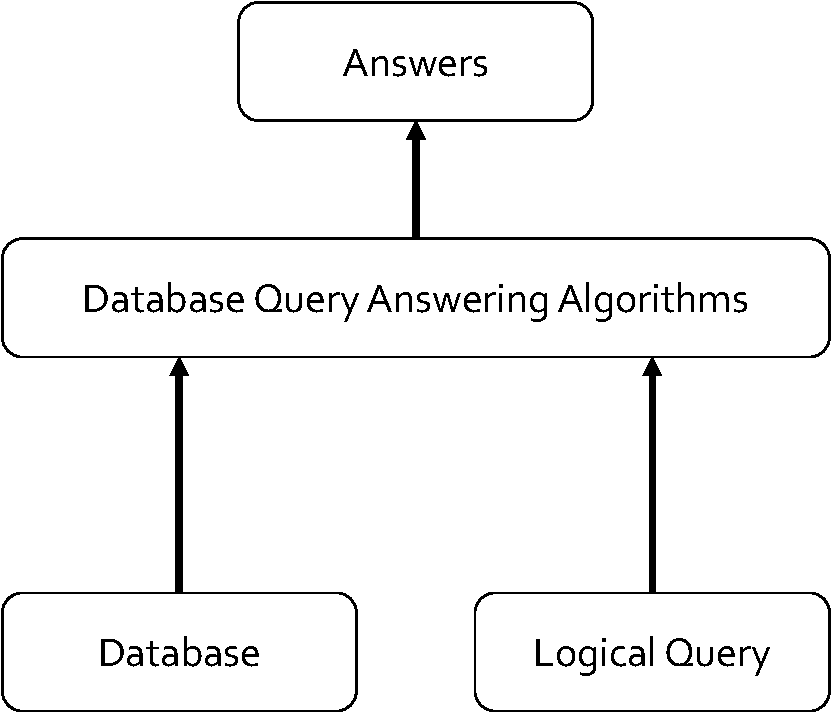
\includegraphics[width=0.31\textwidth]{submissions/logical-queries-survey/fig/paradigm-classic.pdf}
		\label{subfig:dbqa}}
	\end{subfigure}
	\hfill
	\begin{subfigure}[Continuous Query Decomposition ]{
		\centering
		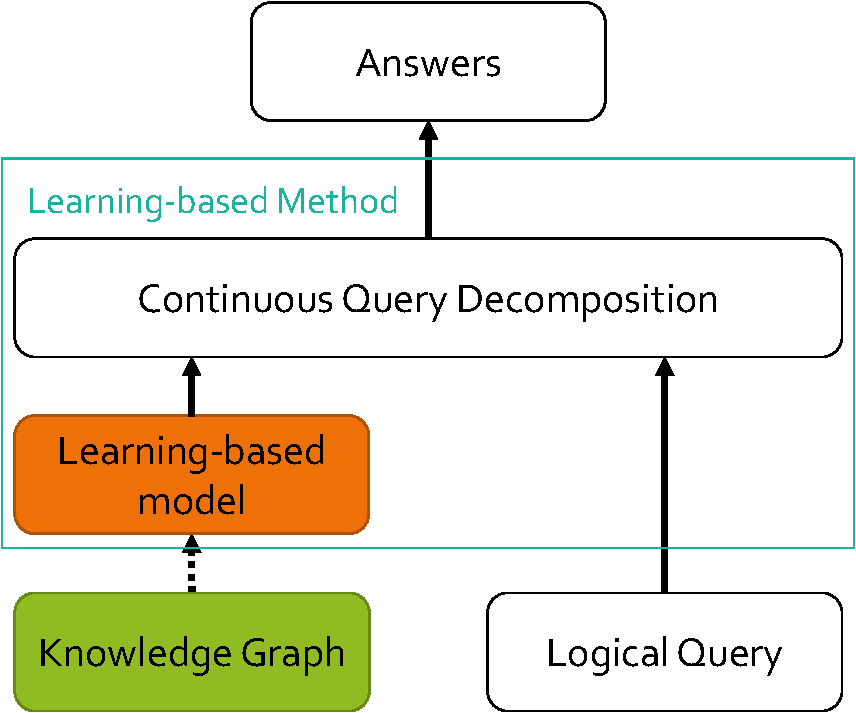
\includegraphics[width=0.31\textwidth]{submissions/logical-queries-survey/fig/paradigm-cqd.pdf}
		\label{subfig:cqd}}
	\end{subfigure}
	\hfill
	\begin{subfigure}[Query Embedding ]{
		\centering
		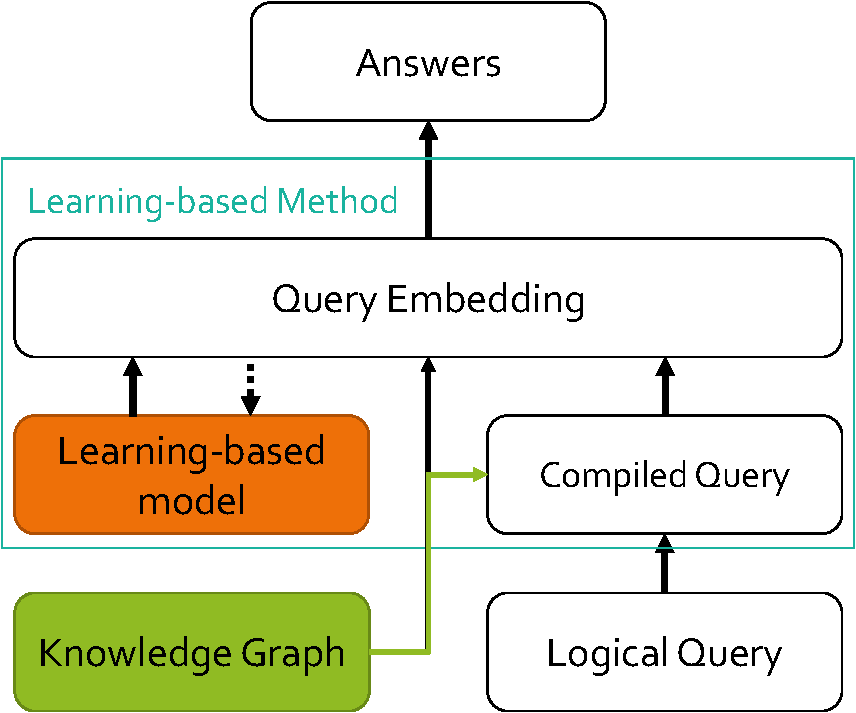
\includegraphics[width=0.31\textwidth]{submissions/logical-queries-survey/fig/paradigm-query-embedding.pdf}
		\label{subfig:query-emb}}
	\end{subfigure}
	\caption{Paradigms for logical query answering on knowledge graphs. The solid line indicates the query answering procedures, and the dashed lines indicate the procedures to obtain the model.}
	\label{fig:old-and-new-paradigms}
\end{figure}


The key to understanding learning-based methods is not only how to define the model but also how models interact with the knowledge graph data and logical queries. The model-query and model-data interaction jointly define the scope of queries that can be answered by each method. Specifically, the model-data interaction refers to how to obtain the model from data, including both training data and algorithms, and the model-query interaction refers to how learning-based models are combined with query answering algorithms. The model-data and model-query interaction are indicated by the dashed arrows and the arrows in Figure~\ref{subfig:cqd} and~\ref{subfig:query-emb}, respectively.


\begin{table}[t]
\small\centering
\caption{Comparison between CQD and QE methods with their training data, query answering algorithms, and solvable queries. $\dag$ indicates that the actual solvable queries may not be the formally defined logical query family.}\label{tab:compare-method}
\begin{tabular}{llrl}
\toprule
Methods                        & Training Data & Query Answering Algorithms & Solvable Queries \\ \midrule
Continuous Query Decomposition (CQD)
  & KG triples                     & Model + Optimization          & EPFO             \\\midrule
\multirow{3}{*}{Query Embedding (QE)} & QA samples & Operator Tree + Model & EFO-1 $^\dag$ \\
                                 & QA samples & Query Graph + Model & EFO-1 $^\dag$ \\
                                 & QA samples & Sequence + Model & EPFO $^\dag$  \\ \bottomrule
\end{tabular}
\end{table}

The rest of this section presents the details of these two types of methods. Table~\ref{tab:compare-method} compares these two types from three aspects, including training data (model-data interaction), query answering algorithms (model-query interaction), and queries that can be solved.
The most distinct difference between CQD and QE is how they treat the model as part of the query answering algorithms.
Continuous query decomposition estimates the answer embedding by solving an optimization problem with continuous objective induced from the original logical formula with logical $t$-norms~\cite{Hajek1998MetamathematicsFuzzy}. This objective, computed by the result of the model inference, will be evaluated multiple times during the optimization process. Therefore, the model will be inferred multiple times. This formulation is denoted as Model + Optimization in Table~\ref{tab:compare-method} where the term Model is placed before Optimization.
In contrast, query embedding methods first compile the logical queries into various representations such as operator trees, query graphs, or sequences. Then, the answer embedding, or the embedding of logical query, is estimated by simple forward inferring the model only once. This formulation is denoted as X + Model, where the term Model is placed after X indicating one of the operator trees, query graphs, or sequences.
As natural consequences of such distinct differences in query answering algorithms, CQD and QE require different types of training data to obtain the model and can solve different types of queries. Moreover, the solvable query families for QE methods differ when the queries are compiled into different representations. We note that the solvable queries are confirmed in existing works, and they can be of course extended to broader classes.

The Disjunctive Normal Form (DNF)~\cite{Marker2002Modeltheory} of the logical queries is of particular interest. This is because (1) all first-order queries can be converted to DNF, and (2) The answer set of DNF existential queries can be regarded as the union of the answer sets of its containing conjunctive clauses. For example, EPFO queries can be answered by compositing the solutions of conjunctive queries. Similarly, general existential logical queries can be answered once the queries with conjunction and negation can be well answered.

\subsection{Continuous Query Decomposition (CQD)}\label{sec:cqd}
The model used in CQD~\cite{Arakelyan2021ComplexQuery} method is no more than a neural link predictor, which is the key part of knowledge graph representaiton~\cite{Zhang2022KnowledgeGraph,Ji2022Surveyknowledge}.
Specifically, CQD leverages the pretrained ComplEx embedding~\cite{Trouillon2016ComplexEmbeddings} and achieves state-of-the-art performances in EPFO queries on dataset~\cite{Ren2020Query2boxReasoning}. The training of the neural link predictor is not related to the logical queries but only knowledge graphs themselves. Recent survey~\cite{Ji2022Surveyknowledge} summarizes the construction of neural link predictors and how to train neural link predictors well is discussed in~\cite{Ruffinelli2020YouCAN}.

CQD uses neural link predictors to solve EPFO queries with a search algorithm. It considers the EPFO query $\phi(v)$ in the following DNF form.
\begin{equation}\label{eq:epfo-cqd}
    \phi(v) = \exists x_1, ..., x_n, (r_{11}\land \cdots \land r_{1k_1}) \lor \cdots \lor (r_{l1}\land \cdots \land r_{lk_l}),
\end{equation}
where $r_ij$ is the atomic formula (without negation) and $v$ is the only free variables associated to one or more $r_ij$.

Once the neural link predictor is obtained, each atomic formula $r(h, t)$ can be evaluated with its probability $p(h, r, t)$ of being true. Let $p_{ij}$ be the probability of $ij$-th triple, $\top$ and $\bot$ be the $t$-norm and $t$-conorm~\cite{Hajek1998MetamathematicsFuzzy}, we rewrite the EPFO query in Equation~(\ref{eq:epfo-cqd}) into the optimization problem:
\begin{equation}\label{eq:objective-cqd}
    \max_{v, x_1, ..., x_n} (p_{11}\top \cdots \top p_{1k_1}) \bot \cdots \bot (p_{l1}\top \cdots \top p_{lk_l}).
\end{equation}
The objective in Problem~(\ref{eq:objective-cqd}) is continuous since $p$, $\top$, and $\bot$ is continuous. Embedding of variables $v, x_1, ..., x_n$ will be optimized over the continuous embedding space with gradient-based optimization or searched on the discrete set $\entity$ with beam-search.
Therefore, complex structures of logical queries are handled by solving the optimization problem with the compositional objective function.
CQD is also applicable to EPFO queries with multiple free variables in principle. However, this is not empirically justified because of the lack of corresponding datasets.
The drawback of CQD is also apparent: CQD eventually estimates the embedding of variables, which remains a significant gap in answering aggregate queries.

\subsection{Query Embedding (QE)}\label{sec:qe}
In contrast to CQD, query embedding methods use explicit representations of the query structures. Direct inference of the learning-based model over specific query representation estimates the embedding of the target variable, i.e., the query embedding. Then the answers can be retrieved according to the query embedding.
The general advantages and disadvantages of QE methods are also clear. On the one hand, models are inferred only once to obtain the answers. On the other hand, specific representation restricts the scope of solvable queries.
In the current stage, there is no dominant representation of the queries. Figure~\ref{fig:query-representation} summarizes popular choices including operator trees~\cite{Wang2021BenchmarkingCombinatorial}, query graphs~\cite{Liu2022MaskReason}, and sequences~\cite{Kotnis2021AnsweringComplex}.
Then we categorize different query embedding methods by their query representations and discuss each type from four perspectives: query representation, model design, training, and query answering algorithms.

\begin{figure}[t]
\centering
    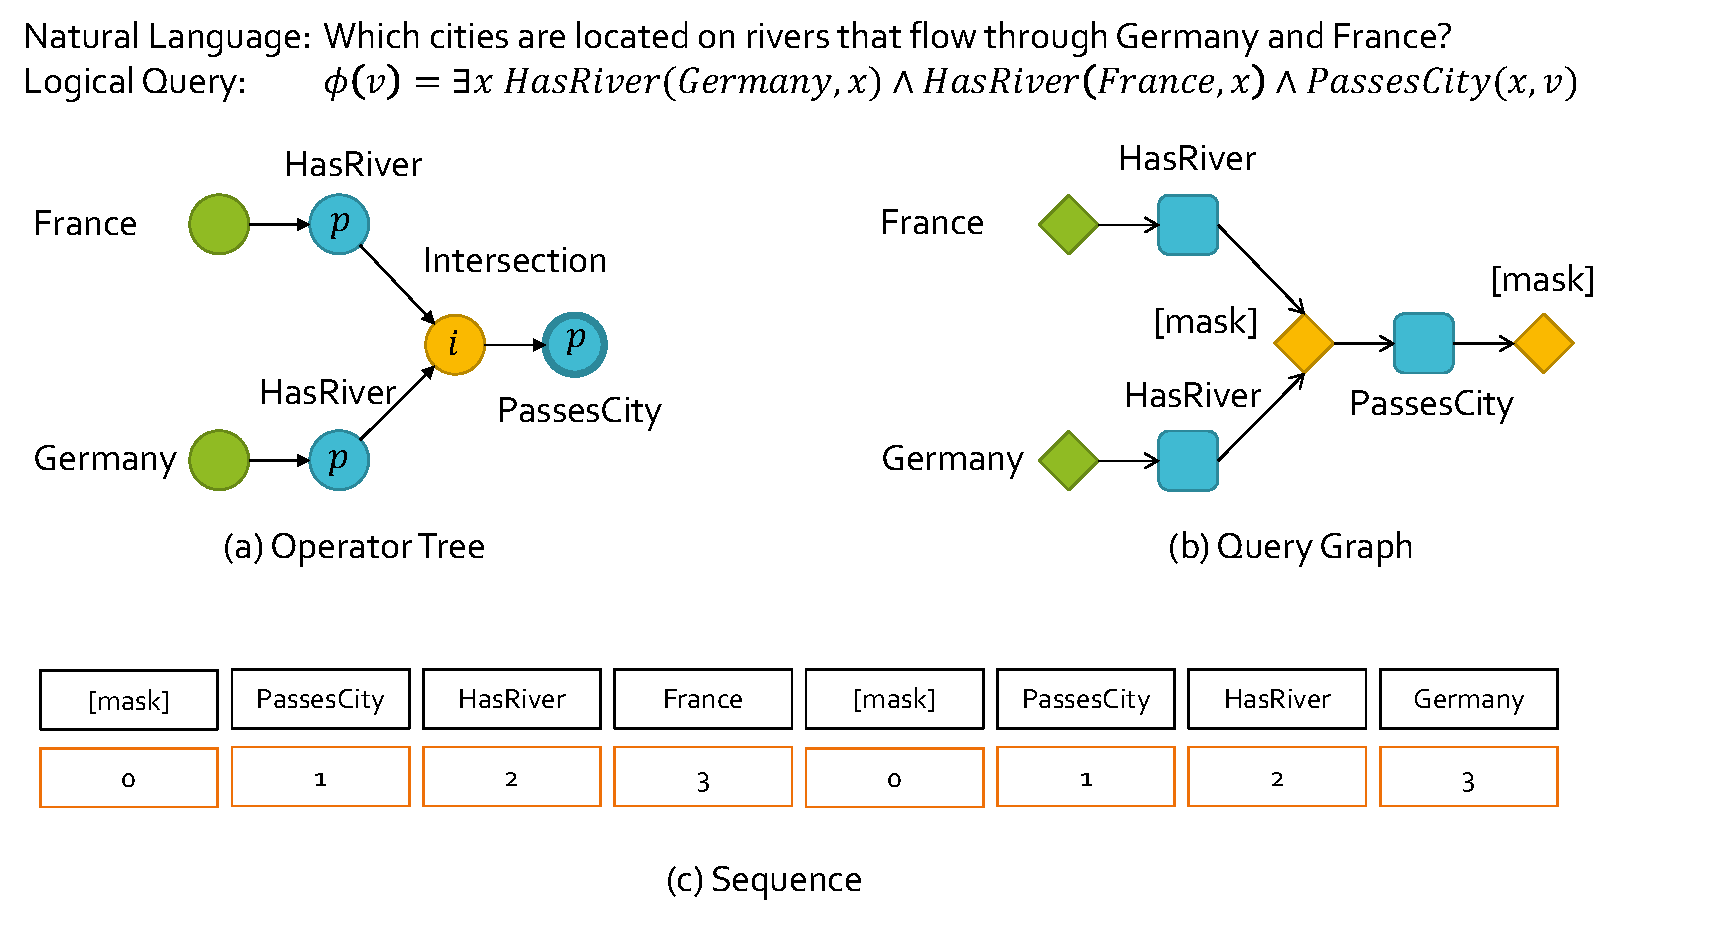
\includegraphics[width=\linewidth]{submissions/logical-queries-survey/fig/logical-query-repr.pdf}
    \caption{Three ways to represent logical query in the query embedding methods. The example is taken from~\cite{Kotnis2021AnsweringComplex}. We see the logical query is converted into three formats, including (a) operator tree~\cite{Wang2021BenchmarkingCombinatorial}, where each node is a set operator; (b) query graph~\cite{Liu2022MaskReason}, where the nodes are terms and predicates; (c) sequences~\cite{Kotnis2021AnsweringComplex}, where a logical query is transformed as the concatenation of several multi-hop queries with a special positional encoding.}\label{fig:query-representation}
\end{figure}

\subsubsection{Logical Queries as Operator Trees}\label{sec:qe-optree}
Operator trees materialize the procedure of searching for answers as the execution of set operators, including set projection, intersection, union, and complement (with respect to a universe).
Each entity itself is regarded as the simplest singleton, a set with only one element.
The set projection is converted from relations by conducting a Skolemization~\cite{Marker2002Modeltheory} process of a logical formula.
Other set operations such as intersection, union, and difference or negation are naturally induced by logical operators.
Only a subset of first-order formulae can be converted into the operator trees because such a representation of logical queries imposes additional assumptions to Definition~\ref{def:formula}, as discussed in~\cite{Wang2021BenchmarkingCombinatorial}.
Meanwhile, the choice of set operators is not identical. For example, the set complement can be replaced by the set difference~\cite{Liu2021NeuralAnsweringLogical}, and the set union can be replaced by intersection and vice versa with the set complement, according to De Morgan's laws.
The learning-based model for operation tree representation is designed to simulate the sets in the continuous embedding spaces and the set simulations with differentiable computations (usually with neural networks). Then we discuss the spaces used to represent sets and the modeling of the set operations.

\noindent\textbf{Geometric Region Embeddings.} Sets, as a collection of discrete objects for logical query answering, are naturally related to the geometrical region of some spaces. Compared to complex variable embeddings as vectors in CQD, embedding sets as geometric regions provides a straightforward estimation of the size of the answer set. The chosen forms of geometric regions are usually simple to be parameterized, such as the boxes used by Query2Box~\cite{Ren2020Query2boxReasoning} and NewLook~\cite{Liu2021NeuralAnsweringLogical}, sector cones two-dimensional spaces used by ConE~\cite{Zhang2021ConECone}, and hyperboloid used by HypE~\cite{Choudhary2021SelfSupervisedHyperboloidc}. The set projection is usually modeled by neural networks that map the parameterized regions to new ones. Intersection and union operators in NewLook are modeled by some variants of deep set network~\cite{Zaheer2017DeepSets} to merge multiple regions into one. Notably, the design of ConE~\cite{Zhang2021ConECone} allows a closed-form set complement with sector cones, while NewLook~\cite{Liu2021NeuralAnsweringLogical} models the set difference between boxes with neural networks. How to handle negation operation using hyperboloid is not yet discussed.

\noindent\textbf{Probabilistic Distribution Embeddings.} Another thread of work models sets with the probabilistic distributions. Parameterized probabilistic distribution families include Beta distribution in BetaE~\cite{Ren2020BetaEmbeddings}, Gaussian distribution in PERM~\cite{Choudhary2021ProbabilisticEntity}, and Gamma distribution in GammaE~\cite{Yang2022GammaEGamma}. Probabilistic distributions are more sophisticated than geometrical regions in set representation because the techniques to construct new probabilistic distributions can be applied to model set operators. For example, a mixture of probabilistic distributions can be used to construct the union operation~\cite{Choudhary2021ProbabilisticEntity,Yang2022GammaEGamma}. Also, altering one parameter to its reciprocal is straightforward to represent the set complement for some family of distributions~\cite{Ren2020BetaEmbeddings,Yang2022GammaEGamma}. Meanwhile, the normalized product of the Probability Distribution Functions (PDF) of Gamma distribution is also Gamma distribution. This fact enables GammaE to simplify the design of the intersection operator. Well-defined distances and divergences between distributions are powerful tools for defining the distances between the answer sets, such as Mahalanobis distance~\cite{Choudhary2021ProbabilisticEntity} and KL-divergence~\cite{Ren2020BetaEmbeddings,Yang2022GammaEGamma}. Following the intuition of probabilistic distributions, LinE~\cite{Huang2022LinELogical} considers the histogram as the unnormalized discretization of arbitrary PDF, and Query2Particles~\cite{Bai2022Query2ParticlesKnowledge} handles a set of empirical samples (particles) from an arbitrary PDF. Such designs sacrifice parts of the closed-form properties but enlarge the family of underlying distributions with non-parametric representations.

\noindent\textbf{Fuzzy Vector Embeddings.} Fuzzy vector space~\cite{Katsaras1977Fuzzyvector} brings supreme advantages in modeling the set operations. Set intersection, union, and negation can be precisely modeled with fuzzy logical $t$-norms and $t$-conorms~\cite{Hajek1998MetamathematicsFuzzy} by embedding sets as fuzzy vectors~\cite{Luus2021LogicEmbeddings,Chen2022FuzzyLogic}, i.e., vectors in $[0, 1]^d$ where $d$ is the dimension. The one thing left is to model the set projections with neural networks. FuzzQE~\cite{Chen2022FuzzyLogic} models the set projection by relational base decomposition~\cite{Schlichtkrull2018ModelingRelational} and LogicE~\cite{Luus2021LogicEmbeddings} uses simple multi-layer perceptron. In addition, LogicE~\cite{Luus2021LogicEmbeddings} models the lower and the upper bounds of the fuzzy logic truth value, which quantifies the uncertainty of each embedding to answer the aggregate query.

In contrast to various designs for embedding spaces, MLPMix~\cite{Amayuelas2022NeuralMethods} just embedded queries as the vectors in the Euclidean space. Such a simple embedding space does not guarantee any set properties, so it requires more advanced neural networks~\cite{tolstikhin2021mlp} to model set operators. Notably, MLPMix still has strong performance with simple embedding space compared to its predecessors. This might suggest that even the simplest Euclidean space is large enough. The overall performance results from the trade-off between set embeddings and set operations.

Neural symbolic methods also shed light on another way to improve performances. ``Neural'' indicates methods answering queries in low-dimensional embedding spaces and neural networks, while ``symbolic'' indicates referring to the original symbolic knowledge graphs. GNN-QE~\cite{Zhu2022NeuralSymbolicModelsa} estimates the probabilities of all entities given the set projection with graph neural network, NBFNet~\cite{Zhu2021NeuralBellmanForda} over the observed knowledge graph. ENeSy~\cite{Xu2022NeuralSymbolicEntangleda} ensembles the neural model prediction and symbolic model prediction at each set projection, where the symbolic part is conducted by the TensorLog~\cite{Cohen2020TensorLogProbabilistic}. These methods show outstanding performances compared to the neural query embedding methods. However, scalability is always an issue since the intermediate states will unavoidably grow with the size of the underlying knowledge graph.

While various models for operator trees were proposed, the method to train the model is almost the same as the first proposed to train Query2box~\cite{Ren2020Query2boxReasoning}. Let $D(e, q)$ be the distance function between the entity $e$ and the query embedding $q$, the objective function is
\begin{equation}
    \ell_\theta(a, q) = -\log \sigma( \gamma - D(a, q) ) - \frac{1}{k} \sum_{i=1}^k \log \sigma( D(v_i,  q) - \gamma),\label{eq:neg-sample}
\end{equation}
where $\sigma = \frac{1}{1+e^{-x}}$ is the sigmoid function, $\gamma$ is the margin, $a$ is an arbitrary answer, and $v_i$ are $k$ negative sampled answers.


\subsubsection{Logical Queries as Query Graphs}
Query graph presentation represents the terms and predicates in to graphs~\cite{Daza2020MessagePassing,Liu2022MaskReason,LMPNN}. Query graph representation does not assume the acyclicity as operator tree representation. Therefore it represents a larger set of logical queries. However, existing query graphs are not related to the disjunction. The disjunction can be handled by converting existing queries to DNF queries, whose answer set is the combination of all conjunctive queries that can be addressed in the query graphs. More specifically, a conjunctive query is represented by two kinds of query graphs: (1) heterogenuous information networks (HIN)~\cite{shi2016survey} where relations and entities are all nodes~\cite{Liu2022MaskReason}; (2) constraint graphs where nodes are terms and edges are atomic formulas~\cite{Arakelyan2021ComplexQuery,LMPNN}. This representation is connected to the constraint programming~\cite{rossi2006handbook}.

The learning-based models for query graphs are basically Graph Neural Networks (GNN). For constraint graph representation, MPQE~\cite{Daza2020MessagePassing} applies message passing networks on EPFO queries and LMPNN~\cite{LMPNN} employs the pretrained knowledge graph embeddings to answer queries with negation.
kgTransformer~\cite{Liu2022MaskReason} uses graph transformers whose multi-layer perceptrons are upgraded by a Mixture of Experts (MoE) architecture. Besides the negative sampling objectives shown in Equation~(\ref{eq:neg-sample}), kgTransformer proposed to first pretrain the model on sampled subgraphs and then finetune the model with the negative sampling loss on query answering data.

\subsubsection{Logical Queries as Sequences}
The last type of representation is to represent the queries in sequences. BiQE~\cite{Kotnis2021AnsweringComplex}, see Figure~\ref{fig:query-representation}~(c), proposes to convert the query graph to multiple paths from the answer node to the anchor entity nodes. Compared to the query graphs, the sequence representation even neglects the existential variables, only the anchor entity and the relations on its path to the answer node remain. Relative positional embeddings are also used to describe the distance from each token to the answer node. This representation also focuses on conjunctive queries, which do not contain disjunction and negation. Queries with disjunctions can be handled by combining conjunctive queries in the DNF. However, it is still not known how to handle the negation operation.

Once the sequence is defined, the sequence can be put into the transformer models. The output embedding of the \texttt{[mask]} token is aggregated to obtain the answer. Unlike the query graph representation that enforces the query structures explicitly, transformers could learn implicit logical structures via the self-attention mechanism.

\section{Future Directions}\label{sec:future}
Research about knowledge graphs logical query answering, though rapidly developed in recent years, is still limited compared to the well-established study about query answering on the relational database. For example, the query types that can be answered by the model are strict fragments of first-order queries.
In this section, we discuss what is left in current research compared to logical query answering on incomplete relational data, which is the ultimate goal of this line of research. Formal definitions from model theory in Section~\ref{sec:data-query} picture the gap between existing works and the ambitious goal. we summarize the limitations and discuss possible future directions from the data, query, and model perspectives.

\subsection{Towards General Relational Data}
A relational language $\lang$ can describe general relational data. However, the language $\lang_{KG}$ for knowledge graphs is defined with three additional assumptions, see Section~\ref{sec:data-query}. By rethinking three assumptions about $\lang_{KG}$ and the open world assumption, we could extend the existing data model of knowledge graphs.

\noindent\textbf{KG with Relations of $n_r > 2$.} Knowledge graphs with $n$-ary relations~\cite{Zhang2022FactTreeReasoning} relax the first assumption that $n_r=2, \forall R\in \relation$ by accepting the relations whose $2\leq n_r \leq n$. Thus, each element of the knowledge graph now is an $n+1$ triple list that contains $n$ entities and one relation. The concept of $n$-ary relation is also related to the hyper-relation~\cite{Galkin2020MessagePassing,Alivanistos2022QueryEmbedding} and the knowledge graph is extended from the directed graphs to hypergraphs.

\noindent\textbf{KG with Attributes.} Attributes expand the constant set $\entity$ from all entities to \textit{entities with attribute values}, thus relaxing the second assumption. Typical attributes include entity types~\cite{Auer2007DBpediaNucleus,Hu2022TypeawareEmbeddings}, triple timestamps~\cite{Jia2021ComplexTemporal,Saxena2021QuestionAnswering}, and triple probabilities~\cite{Carlson2010ArchitectureNeverEnding}. Additional attributes can be described in the $n$-ary relations. For example, the timestamp $t$ associated with a triple $(s, p, o)$ can be described with 4-triples $(s, p, o, t)$. New attributes bring new predicates, enlarge the universe set, and enrich the query semantics. Two timestamps can be compared by ``before'', ``equal'', and ``after'', and can be composed to a time interval, which also introduces new predicates such as ``during''. The triple probabilities, as discussed in probabilistic databases~\cite{VandenBroeck2017QueryProcessing}, enable the estimation of the probabilities for boolean queries, the probability for each answer entity for set-valued queries, and the total probability for aggregate queries.

\noindent\textbf{KG with Functions.} Introducing attributes also makes it possible to define functions between attribute values. Taking the timestamp attribute as an example, new timestamps can be computed by a time movement function with a timestamp and a time interval as inputs. These features are rigorously defined in pure symbolic systems~\cite{emerson1990temporal}. It is worth discussing how to combine them with learning-based methods.

\noindent\textbf{More Challenging Open World Assumption.}  In the inductive setting, the entity set $\entity$ is divided into an observed set $\entity_o^r$ and an inempty inductive set $\entity_i^r$ with respect to the relation $r\in \relation$, that is $\entity_o^r\cap\entity_i^r = \emptyset, \entity_o^r\cup\entity_i^r = \entity, \forall r\in\relation$. Under such a setting, the open world assumption in Definition~\ref{def:owa} is rewritten as $I_{\kgnew_o}(r) \subseteq \entity_o^r\times \entity_o^r \subseteq I_{\kgnew_u}(r) \subseteq \entity\times \entity$. This setting makes it very hard to estimate the relations over $\entity\times \entity - \entity_o^r\times \entity_o^r $.
% \begin{compactitem}
%     \item
%     \item
%     \item Temporal information~\cite{jia2021ComplexTemporalQuestion,saxena2021QuestionAnsweringTemporal},
%      we extend the language $\lang$ so that the entity set $\entity$ contains not only  all entities in the knowledge graph but also all possible timestamps which are real numbers. This extension induces additional predicates in the $\relation$ set, such as ``before", ``during'', and ``next'', which can be interpreted as corresponding predicates defined by the real axis. More importantly, this makes  $\entity$ an infinite set since it includes the set of real numbers $R$, which greatly differs from the original settings of the finite language defined by the finite knowledge graph. On the other hand, spatial information doesn't induce the infinite problem and is thus omitted in our discussion.
% \end{compactitem}

\subsection{Towards First Order Queries and Beyond}
The semantics of the logic queries lacks serious discussion. There is no standard dataset and benchmark for first-order queries with cycles, multiple free variables, or universal quantifiers even for the simplest $L_{KG}$ language. Moreover, it is also worth discussing first-order queries over general relational data such as KGs with attributes and attribute functions. It is also worthwhile to expand the first-order logic to fixed-point or monadic second-order logic~\cite{Libkin2004ElementsFinite}.

\subsection{Towards Versatile Learning-based Models}
Existing methods are incapable of addressing more and more challenging queries and complex data discussed above. It is essential to investigate the graph or sequence-based query embedding models to solve various queries. Given the combinatorial natures of the query answering problems, new opportunities could be found with neural combinatorial solvers~\cite{DBLP:conf/iclr/BelloPL0B17}. Meanwhile, large language models, as a proven effective way to encapsulate world knowledge~\cite{petroni2019language,brown2020language}, could be considered as another approach to modeling the relational data.

\section{Conclusion}
Big data and world knowledge are usually uncertain and dynamic. Logical queries over knowledge graphs are essential ways to understand the world as a simplified data model through the lens of logic and reasoning.
In this paper, we structure the existing knowledge graph logical query answering tasks and methods as a three-party game between data, query, and models. With the rigorous concepts from finite model theory~\cite{Marker2002Modeltheory,Libkin2004ElementsFinite}, our work portrays a detailed landscape of the achievements and limitations of existing work. Our discussion shows that there are various gaps between current research to the ambitious goal in terms of data, queries, and models. We hope our paper can be a practical guide for traveling in the uncertain and dynamic data world.

\section{Ackonwledgement}
The authors of this paper were supported by the NSFC Fund (U20B2053) from the NSFC of China, the RIF (R6020-19 and R6021-20) and the GRF (16211520 and 16205322) from RGC of Hong Kong, the MHKJFS (MHP/001/19) from ITC of Hong Kong and the National Key R\&D Program of China (2019YFE0198200) with special thanks to HKMAAC and CUSBLT, and the Jiangsu Province Science and Technology Collaboration Fund (BZ2021065). We also thank the support from NVIDIA AI Technology Center (NVAITC) and the UGC Research Matching Grants (RMGS20EG01-D, RMGS20CR11, RMGS20CR12, RMGS20EG19, RMGS20EG21, RMGS23CR05, RMGS23EG08).

%\bibliographystyle{plain}
%\bibliography{submissions/logical-queries-survey/ref}
%\bibliographystyle{plain}
%\bibliography{submissions/causal-meta-knowledge/sample}


\begin{thebibliography}{10}

\bibitem{abiteboul1995FoundationsDatabases}
S.~Abiteboul, Richard Hull, and Victor Vianu.
\newblock {\em Foundations of Databases}.
\newblock {Addison-Wesley}, {Reading, Mass}, 1995.

\bibitem{Alivanistos2022QueryEmbedding}
Dimitrios Alivanistos, Max Berrendorf, Michael Cochez, and Mikhail Galkin.
\newblock Query {{Embedding}} on {{Hyper-Relational Knowledge Graphs}}.
\newblock In {\em International {{Conference}} on {{Learning
  Representations}}}, March 2022.

\bibitem{Amayuelas2022NeuralMethods}
Alfonso Amayuelas, Shuai Zhang, Susie~Xi Rao, and Ce~Zhang.
\newblock Neural {{Methods}} for {{Logical Reasoning}} over {{Knowledge
  Graphs}}.
\newblock In {\em The {{Tenth International Conference}} on {{Learning
  Representations}}, {{ICLR}} 2022, {{Virtual Event}}, {{April}} 25-29, 2022}.
  {OpenReview.net}, 2022.

\bibitem{Arakelyan2021ComplexQuery}
Erik Arakelyan, Daniel Daza, Pasquale Minervini, and Michael Cochez.
\newblock Complex {{Query Answering}} with {{Neural Link Predictors}}.
\newblock In {\em International {{Conference}} on {{Learning
  Representations}}}, 2021.

\bibitem{Auer2007DBpediaNucleus}
S{\"o}ren Auer, Christian Bizer, Georgi Kobilarov, Jens Lehmann, Richard
  Cyganiak, and Zachary Ives.
\newblock {{DBpedia}}: {{A Nucleus}} for a {{Web}} of {{Open Data}}.
\newblock In Karl Aberer, Key-Sun Choi, Natasha Noy, Dean Allemang, Kyung-Il
  Lee, Lyndon Nixon, Jennifer Golbeck, Peter Mika, Diana Maynard, Riichiro
  Mizoguchi, Guus Schreiber, and Philippe {Cudr{\'e}-Mauroux}, editors, {\em
  The {{Semantic Web}}}, Lecture {{Notes}} in {{Computer Science}}, pages
  722--735, {Berlin, Heidelberg}, 2007. {Springer}.

\bibitem{Bai2022Query2ParticlesKnowledge}
Jiaxin Bai, Zihao Wang, Hongming Zhang, and Yangqiu Song.
\newblock {{Query2Particles}}: {{Knowledge Graph Reasoning}} with {{Particle
  Embeddings}}.
\newblock In {\em Findings of the {{Association}} for {{Computational
  Linguistics}}: {{NAACL}} 2022}, pages 2703--2714, {Seattle, United States},
  July 2022. {Association for Computational Linguistics}.

\bibitem{DBLP:conf/iclr/BelloPL0B17}
Irwan Bello, Hieu Pham, Quoc~V. Le, Mohammad Norouzi, and Samy Bengio.
\newblock Neural combinatorial optimization with reinforcement learning.
\newblock In {\em 5th International Conference on Learning Representations,
  {ICLR} 2017, Toulon, France, April 24-26, 2017, Workshop Track Proceedings}.
  OpenReview.net, 2017.

\bibitem{Bollacker2008Freebasecollaboratively}
Kurt~D. Bollacker, Colin Evans, Praveen~K. Paritosh, Tim Sturge, and Jamie
  Taylor.
\newblock Freebase: A collaboratively created graph database for structuring
  human knowledge.
\newblock In Jason Tsong-Li Wang, editor, {\em Proceedings of the {{ACM SIGMOD
  International Conference}} on {{Management}} of {{Data}}, {{SIGMOD}} 2008,
  {{Vancouver}}, {{BC}}, {{Canada}}, {{June}} 10-12, 2008}, pages 1247--1250.
  {ACM}, 2008.

\bibitem{Bordes2013TranslatingEmbeddings}
Antoine Bordes, Nicolas Usunier, Alberto {Garcia-Duran}, Jason Weston, and
  Oksana Yakhnenko.
\newblock Translating {{Embeddings}} for {{Modeling Multi-relational Data}}.
\newblock In {\em Advances in {{Neural Information Processing Systems}}},
  volume~26. {Curran Associates, Inc.}, 2013.

\bibitem{brown2020language}
Tom Brown, Benjamin Mann, Nick Ryder, Melanie Subbiah, Jared~D Kaplan, Prafulla
  Dhariwal, Arvind Neelakantan, Pranav Shyam, Girish Sastry, Amanda Askell,
  et~al.
\newblock Language models are few-shot learners.
\newblock {\em Advances in neural information processing systems},
  33:1877--1901, 2020.

\bibitem{Carlson2010ArchitectureNeverEnding}
Andrew Carlson, Justin Betteridge, Bryan Kisiel, Burr Settles, Estevam
  R.~Hruschka Jr, and Tom~M. Mitchell.
\newblock Toward an {{Architecture}} for {{Never-Ending Language Learning}}.
\newblock In Maria Fox and David Poole, editors, {\em Proceedings of the
  {{Twenty-Fourth AAAI Conference}} on {{Artificial Intelligence}}, {{AAAI}}
  2010, {{Atlanta}}, {{Georgia}}, {{USA}}, {{July}} 11-15, 2010}. {AAAI Press},
  2010.

\bibitem{Chen2022FuzzyLogic}
Xuelu Chen, Ziniu Hu, and Yizhou Sun.
\newblock Fuzzy {{Logic Based Logical Query Answering}} on {{Knowledge
  Graphs}}.
\newblock In {\em Thirty-{{Sixth AAAI Conference}} on {{Artificial
  Intelligence}}, {{AAAI}} 2022, {{Thirty-Fourth Conference}} on {{Innovative
  Applications}} of {{Artificial Intelligence}}, {{IAAI}} 2022, {{The Twelveth
  Symposium}} on {{Educational Advances}} in {{Artificial Intelligence}},
  {{EAAI}} 2022 {{Virtual Event}}, {{February}} 22 - {{March}} 1, 2022}, pages
  3939--3948. {AAAI Press}, 2022.

\bibitem{Choudhary2021ProbabilisticEntity}
Nurendra Choudhary, Nikhil Rao, Sumeet Katariya, Karthik Subbian, and Chandan
  Reddy.
\newblock Probabilistic {{Entity Representation Model}} for {{Reasoning}} over
  {{Knowledge Graphs}}.
\newblock In {\em Advances in {{Neural Information Processing Systems}}},
  volume~34, pages 23440--23451. {Curran Associates, Inc.}, 2021.

\bibitem{Choudhary2021SelfSupervisedHyperboloidc}
Nurendra Choudhary, Nikhil Rao, Sumeet Katariya, Karthik Subbian, and
  Chandan~K. Reddy.
\newblock Self-{{Supervised Hyperboloid Representations}} from {{Logical
  Queries}} over {{Knowledge Graphs}}.
\newblock In {\em Proceedings of the {{Web Conference}} 2021}, {{WWW}} '21,
  pages 1373--1384, {New York, NY, USA}, June 2021. {Association for Computing
  Machinery}.

\bibitem{Cohen2020TensorLogProbabilistic}
William Cohen, Fan Yang, and Kathryn~Rivard Mazaitis.
\newblock {{TensorLog}}: {{A Probabilistic Database Implemented Using
  Deep-Learning Infrastructure}}.
\newblock {\em Journal of Artificial Intelligence Research}, 67:285--325,
  February 2020.

\bibitem{Daza2020MessagePassing}
Daniel Daza and Michael Cochez.
\newblock Message {{Passing Query Embedding}}, June 2020.

\bibitem{emerson1990temporal}
E~Allen Emerson.
\newblock Temporal and modal logic.
\newblock In {\em Formal Models and Semantics}, pages 995--1072. Elsevier,
  1990.

\bibitem{Galkin2020MessagePassing}
Mikhail Galkin, Priyansh Trivedi, Gaurav Maheshwari, Ricardo Usbeck, and Jens
  Lehmann.
\newblock Message {{Passing}} for {{Hyper-Relational Knowledge Graphs}}.
\newblock In {\em Proceedings of the 2020 {{Conference}} on {{Empirical
  Methods}} in {{Natural Language Processing}} ({{EMNLP}})}, pages 7346--7359,
  {Online}, November 2020. {Association for Computational Linguistics}.

\bibitem{Galkin2022InductiveLogical}
Mikhail Galkin, Zhaocheng Zhu, Hongyu Ren, and Jian Tang.
\newblock Inductive {{Logical Query Answering}} in {{Knowledge Graphs}}.
\newblock In {\em Advances in {{Neural Information Processing Systems}} 33:
  {{Annual Conference}} on {{Neural Information Processing Systems}} 2022
  {{NeurIPS}} 2022, {{November}} 27- {{December}} 9, 2022, {{New Orleans}}},
  page~25, 2022.

\bibitem{Hajek1998MetamathematicsFuzzy}
Petr H{\'a}jek.
\newblock {\em Metamathematics of {{Fuzzy Logic}}}, volume~4 of {\em Trends in
  {{Logic}}}.
\newblock {Springer Netherlands}, {Dordrecht}, 1998.

\bibitem{Hamilton2018EmbeddingLogical}
William~L. Hamilton, Payal Bajaj, Marinka Zitnik, Dan Jurafsky, and Jure
  Leskovec.
\newblock Embedding {{Logical Queries}} on {{Knowledge Graphs}}.
\newblock In Samy Bengio, Hanna~M. Wallach, Hugo Larochelle, Kristen Grauman,
  Nicol{\`o} {Cesa-Bianchi}, and Roman Garnett, editors, {\em Advances in
  {{Neural Information Processing Systems}} 31: {{Annual Conference}} on
  {{Neural Information Processing Systems}} 2018, {{NeurIPS}} 2018,
  {{December}} 3-8, 2018, {{Montr\'eal}}, {{Canada}}}, pages 2030--2041, 2018.

\bibitem{Hu2020OpenGraph}
Weihua Hu, Matthias Fey, Marinka Zitnik, Yuxiao Dong, Hongyu Ren, Bowen Liu,
  Michele Catasta, and Jure Leskovec.
\newblock Open {{Graph Benchmark}}: {{Datasets}} for {{Machine Learning}} on
  {{Graphs}}.
\newblock In {\em Advances in {{Neural Information Processing Systems}}},
  volume~33, pages 22118--22133. {Curran Associates, Inc.}, 2020.

\bibitem{Hu2022TypeawareEmbeddings}
Zhiwei Hu, Victor Gutierrez~Basulto, Zhiliang Xiang, Xiaoli Li, Ru~Li, and Jeff
  Z.~Pan.
\newblock Type-aware {{Embeddings}} for {{Multi-Hop Reasoning}} over
  {{Knowledge Graphs}}.
\newblock In {\em Proceedings of the {{Thirty-First International Joint
  Conference}} on {{Artificial Intelligence}}}, pages 3078--3084, {Vienna,
  Austria}, July 2022. {International Joint Conferences on Artificial
  Intelligence Organization}.

\bibitem{Huang2022LinELogical}
Zijian Huang, Meng-Fen Chiang, and Wang-Chien Lee.
\newblock {{LinE}}: {{Logical Query Reasoning}} over {{Hierarchical Knowledge
  Graphs}}.
\newblock In {\em Proceedings of the 28th {{ACM SIGKDD Conference}} on
  {{Knowledge Discovery}} and {{Data Mining}}}, {{KDD}} '22, pages 615--625,
  {New York, NY, USA}, August 2022. {Association for Computing Machinery}.

\bibitem{Ji2022Surveyknowledge}
Shaoxiong Ji, Shirui Pan, Erik Cambria, Pekka Marttinen, and Philip~S. Yu.
\newblock A survey on knowledge graphs: Representation, acquisition, and
  applications.
\newblock {\em IEEE Transactions on Neural Networks and Learning Systems},
  33(2):494--514, February 2022.

\bibitem{Jia2021ComplexTemporal}
Zhen Jia, Soumajit Pramanik, Rishiraj~Saha Roy, and Gerhard Weikum.
\newblock Complex {{Temporal Question Answering}} on {{Knowledge Graphs}}.
\newblock In Gianluca Demartini, Guido Zuccon, J.~Shane Culpepper, Zi~Huang,
  and Hanghang Tong, editors, {\em {{CIKM}} '21: {{The}} 30th {{ACM
  International Conference}} on {{Information}} and {{Knowledge Management}},
  {{Virtual Event}}, {{Queensland}}, {{Australia}}, {{November}} 1 - 5, 2021},
  pages 792--802. {ACM}, 2021.

\bibitem{Katsaras1977Fuzzyvector}
A.~K Katsaras and D.~B Liu.
\newblock Fuzzy vector spaces and fuzzy topological vector spaces.
\newblock {\em Journal of Mathematical Analysis and Applications},
  58(1):135--146, March 1977.

\bibitem{Kotnis2021AnsweringComplex}
Bhushan Kotnis, Carolin Lawrence, and Mathias Niepert.
\newblock Answering {{Complex Queries}} in {{Knowledge Graphs}} with
  {{Bidirectional Sequence Encoders}}.
\newblock {\em Proceedings of the AAAI Conference on Artificial Intelligence},
  35(6):4968--4977, May 2021.

\bibitem{Kroenke2018Databaseprocessing}
David~M. Kroenke, David~J. Auer, Scott~L. Vandenberg, and Robert~C. Yoder.
\newblock {\em Database Processing: Fundamentals, Design, and Implementation}.
\newblock {Pearson}, {NY NY}, 15th edition, 40th anniversary edition edition,
  2018.

\bibitem{Libkin2004ElementsFinite}
Leonid Libkin.
\newblock {\em Elements of {{Finite Model Theory}}}.
\newblock {Springer Berlin Heidelberg}, {Berlin, Heidelberg}, 2004.

\bibitem{Libkin2009OpenClosed}
Leonid Libkin and Cristina Sirangelo.
\newblock Open and {{Closed World Assumptions}} in {{Data Exchange}}.
\newblock In Bernardo~Cuenca Grau, Ian Horrocks, Boris Motik, and Ulrike
  Sattler, editors, {\em Proceedings of the 22nd {{International Workshop}} on
  {{Description Logics}} ({{DL}} 2009), {{Oxford}}, {{UK}}, {{July}} 27-30,
  2009}, volume 477 of {\em {{CEUR Workshop Proceedings}}}. {CEUR-WS.org},
  2009.

\bibitem{Lin2019KagNetKnowledgeAware}
Bill~Yuchen Lin, Xinyue Chen, Jamin Chen, and Xiang Ren.
\newblock {{KagNet}}: {{Knowledge-Aware Graph Networks}} for {{Commonsense
  Reasoning}}.
\newblock {\em EMNLP/IJCNLP}, 2019.

\bibitem{Liu2021NeuralAnsweringLogical}
Lihui Liu, Boxin Du, Heng Ji, ChengXiang Zhai, and Hanghang Tong.
\newblock Neural-{{Answering Logical Queries}} on {{Knowledge Graphs}}.
\newblock In {\em Proceedings of the 27th {{ACM SIGKDD Conference}} on
  {{Knowledge Discovery}} \& {{Data Mining}}}, {{KDD}} '21, pages 1087--1097,
  {New York, NY, USA}, August 2021. {Association for Computing Machinery}.

\bibitem{Liu2022MaskReason}
Xiao Liu, Shiyu Zhao, Kai Su, Yukuo Cen, Jiezhong Qiu, Mengdi Zhang, Wei Wu,
  Yuxiao Dong, and Jie Tang.
\newblock Mask and {{Reason}}: {{Pre-Training Knowledge Graph Transformers}}
  for {{Complex Logical Queries}}.
\newblock In {\em Proceedings of the 28th {{ACM SIGKDD Conference}} on
  {{Knowledge Discovery}} and {{Data Mining}}}, {{KDD}} '22, pages 1120--1130,
  {New York, NY, USA}, August 2022. {Association for Computing Machinery}.

\bibitem{Luus2021LogicEmbeddings}
Francois Luus, Prithviraj Sen, Pavan Kapanipathi, Ryan Riegel, Ndivhuwo
  Makondo, Thabang Lebese, and Alexander Gray.
\newblock Logic {{Embeddings}} for {{Complex Query Answering}}.
\newblock {\em arXiv:2103.00418 [cs]}, February 2021.

\bibitem{Marker2002Modeltheory}
D.~Marker.
\newblock {\em Model Theory: An Introduction}.
\newblock Number 217 in Graduate Texts in Mathematics. {Springer}, {New York},
  2002.

\bibitem{Miller1995WordNetlexical}
George~A. Miller.
\newblock {{WordNet}}: A lexical database for {{English}}.
\newblock {\em Communications of the ACM}, 38(11):39--41, November 1995.

\bibitem{PellissierTanon2016FreebaseWikidata}
Thomas Pellissier~Tanon, Denny Vrande{\v c}i{\'c}, Sebastian Schaffert, Thomas
  Steiner, and Lydia Pintscher.
\newblock From {{Freebase}} to {{Wikidata}}: {{The Great Migration}}.
\newblock In {\em Proceedings of the 25th {{International Conference}} on
  {{World Wide Web}}}, {{WWW}} '16, pages 1419--1428, {Republic and Canton of
  Geneva, CHE}, April 2016. {International World Wide Web Conferences Steering
  Committee}.

\bibitem{petroni2019language}
Fabio Petroni, Tim Rockt{\"a}schel, Sebastian Riedel, Patrick Lewis, Anton
  Bakhtin, Yuxiang Wu, and Alexander Miller.
\newblock Language models as knowledge bases?
\newblock In {\em Proceedings of the 2019 Conference on Empirical Methods in
  Natural Language Processing and the 9th International Joint Conference on
  Natural Language Processing (EMNLP-IJCNLP)}, pages 2463--2473, 2019.

\bibitem{Ren2021LEGOLatent}
Hongyu Ren, Hanjun Dai, Bo~Dai, Xinyun Chen, Michihiro Yasunaga, Haitian Sun,
  Dale Schuurmans, Jure Leskovec, and Denny Zhou.
\newblock {{LEGO}}: {{Latent Execution-Guided Reasoning}} for {{Multi-Hop
  Question Answering}} on {{Knowledge Graphs}}.
\newblock In {\em Proceedings of the 38th {{International Conference}} on
  {{Machine Learning}}}, pages 8959--8970. {PMLR}, July 2021.

\bibitem{Ren2022SMOREKnowledgea}
Hongyu Ren, Hanjun Dai, Bo~Dai, Xinyun Chen, Denny Zhou, Jure Leskovec, and
  Dale Schuurmans.
\newblock {{SMORE}}: {{Knowledge Graph Completion}} and {{Multi-hop Reasoning}}
  in {{Massive Knowledge Graphs}}.
\newblock In {\em Proceedings of the 28th {{ACM SIGKDD Conference}} on
  {{Knowledge Discovery}} and {{Data Mining}}}, {{KDD}} '22, pages 1472--1482,
  {New York, NY, USA}, August 2022. {Association for Computing Machinery}.

\bibitem{Ren2020Query2boxReasoning}
Hongyu Ren, Weihua Hu, and Jure Leskovec.
\newblock Query2box: {{Reasoning}} over {{Knowledge Graphs}} in {{Vector Space
  Using Box Embeddings}}.
\newblock In {\em 8th {{International Conference}} on {{Learning
  Representations}}, {{ICLR}} 2020, {{Addis Ababa}}, {{Ethiopia}}, {{April}}
  26-30, 2020}. {OpenReview.net}, 2020.

\bibitem{Ren2020BetaEmbeddings}
Hongyu Ren and Jure Leskovec.
\newblock Beta {{Embeddings}} for {{Multi-Hop Logical Reasoning}} in
  {{Knowledge Graphs}}.
\newblock In Hugo Larochelle, Marc'Aurelio Ranzato, Raia Hadsell, Maria-Florina
  Balcan, and Hsuan-Tien Lin, editors, {\em Advances in {{Neural Information
  Processing Systems}} 33: {{Annual Conference}} on {{Neural Information
  Processing Systems}} 2020, {{NeurIPS}} 2020, {{December}} 6-12, 2020,
  Virtual}, 2020.

\bibitem{rossi2006handbook}
Francesca Rossi, Peter Van~Beek, and Toby Walsh.
\newblock {\em Handbook of constraint programming}.
\newblock Elsevier, 2006.

\bibitem{Ruffinelli2020YouCAN}
Daniel Ruffinelli, Samuel Broscheit, and Rainer Gemulla.
\newblock You {{CAN Teach}} an {{Old Dog New Tricks}}! {{On Training Knowledge
  Graph Embeddings}}.
\newblock In {\em International {{Conference}} on {{Learning
  Representations}}}, March 2020.

\bibitem{Saxena2021QuestionAnswering}
Apoorv Saxena, Soumen Chakrabarti, and Partha~P. Talukdar.
\newblock Question {{Answering Over Temporal Knowledge Graphs}}.
\newblock In Chengqing Zong, Fei Xia, Wenjie Li, and Roberto Navigli, editors,
  {\em Proceedings of the 59th {{Annual Meeting}} of the {{Association}} for
  {{Computational Linguistics}} and the 11th {{International Joint Conference}}
  on {{Natural Language Processing}}, {{ACL}}/{{IJCNLP}} 2021, ({{Volume}} 1:
  {{Long Papers}}), {{Virtual Event}}, {{August}} 1-6, 2021}, pages 6663--6676.
  {Association for Computational Linguistics}, 2021.

\bibitem{Schlichtkrull2018ModelingRelational}
Michael Schlichtkrull, Thomas~N. Kipf, Peter Bloem, Rianne {van~den Berg}, Ivan
  Titov, and Max Welling.
\newblock Modeling {{Relational Data}} with {{Graph Convolutional Networks}}.
\newblock In Aldo Gangemi, Roberto Navigli, Maria-Esther Vidal, Pascal Hitzler,
  Rapha{\"e}l Troncy, Laura Hollink, Anna Tordai, and Mehwish Alam, editors,
  {\em The {{Semantic Web}}}, Lecture {{Notes}} in {{Computer Science}}, pages
  593--607, {Cham}, 2018. {Springer International Publishing}.

\bibitem{shi2016survey}
Chuan Shi, Yitong Li, Jiawei Zhang, Yizhou Sun, and S~Yu Philip.
\newblock A survey of heterogeneous information network analysis.
\newblock {\em IEEE Transactions on Knowledge and Data Engineering},
  29(1):17--37, 2016.

\bibitem{Sun2022JointLKJoint}
Yueqing Sun, Qi~Shi, Le~Qi, and Yu~Zhang.
\newblock {{JointLK}}: {{Joint Reasoning}} with {{Language Models}} and
  {{Knowledge Graphs}} for {{Commonsense Question Answering}}.
\newblock In Marine Carpuat, Marie-Catherine de~Marneffe, and Iv{\'a}n
  Vladimir~Meza Ru{\'i}z, editors, {\em Proceedings of the 2022 {{Conference}}
  of the {{North American Chapter}} of the {{Association}} for {{Computational
  Linguistics}}: {{Human Language Technologies}}, {{NAACL}} 2022, {{Seattle}},
  {{WA}}, {{United States}}, {{July}} 10-15, 2022}, pages 5049--5060.
  {Association for Computational Linguistics}, 2022.

\bibitem{Talmor2018WebKnowledgeBase}
Alon Talmor and Jonathan Berant.
\newblock The {{Web}} as a {{Knowledge-Base}} for {{Answering Complex
  Questions}}.
\newblock In {\em Proceedings of the 2018 {{Conference}} of the {{North
  American Chapter}} of the {{Association}} for {{Computational Linguistics}}:
  {{Human Language Technologies}}, {{Volume}} 1 ({{Long Papers}})}, pages
  641--651, {New Orleans, Louisiana}, June 2018. {Association for Computational
  Linguistics}.

\bibitem{Teru2020InductiveRelation}
Komal Teru, Etienne Denis, and William~L Hamilton.
\newblock Inductive {{Relation Prediction}} by {{Subgraph Reasoning}}.
\newblock In {\em Proceedings of the 37th {{International Conference}} on
  {{Machine Learning}}}, pages 9448--9457. {PMLR}, November 2020.

\bibitem{tolstikhin2021mlp}
Ilya~O Tolstikhin, Neil Houlsby, Alexander Kolesnikov, Lucas Beyer, Xiaohua
  Zhai, Thomas Unterthiner, Jessica Yung, Andreas Steiner, Daniel Keysers,
  Jakob Uszkoreit, et~al.
\newblock Mlp-mixer: An all-mlp architecture for vision.
\newblock {\em Advances in Neural Information Processing Systems},
  34:24261--24272, 2021.

\bibitem{Toutanova2015Observedlatent}
Kristina Toutanova and Danqi Chen.
\newblock Observed versus latent features for knowledge base and text
  inference.
\newblock In {\em Proceedings of the 3rd {{Workshop}} on {{Continuous Vector
  Space Models}} and Their {{Compositionality}}}, pages 57--66, {Beijing,
  China}, July 2015. {Association for Computational Linguistics}.

\bibitem{Trouillon2016ComplexEmbeddings}
Th{\'e}o Trouillon, Johannes Welbl, Sebastian Riedel, Eric Gaussier, and
  Guillaume Bouchard.
\newblock Complex {{Embeddings}} for {{Simple Link Prediction}}.
\newblock In {\em Proceedings of {{The}} 33rd {{International Conference}} on
  {{Machine Learning}}}, pages 2071--2080. {PMLR}, June 2016.

\bibitem{VandenBroeck2017QueryProcessing}
Guy {Van den Broeck} and Dan Suciu.
\newblock Query {{Processing}} on {{Probabilistic Data}}: {{A Survey}}.
\newblock {\em Foundations and Trends\textregistered{} in Databases},
  7(3-4):197--341, 2017.

\bibitem{Vrandecic2014Wikidatafree}
Denny Vrande{\v c}i{\'c} and Markus Kr{\"o}tzsch.
\newblock Wikidata: A free collaborative knowledgebase.
\newblock {\em Communications of the ACM}, 57(10):78--85, September 2014.

\bibitem{LMPNN}
Zihao Wang, Yangqiu Song, Ginny~Y. Wong, and Simon See.
\newblock Logical message passing networks with one-hop inference on atomic
  formulas.
\newblock In {\em The Eleventh International Conference on Learning
  Representations, {ICLR} 2023, Kigali Rwanda, May 1-5, 2023}. OpenReview.net,
  2023.

\bibitem{Wang2021BenchmarkingCombinatorial}
Zihao Wang, Hang Yin, and Yangqiu Song.
\newblock Benchmarking the {{Combinatorial Generalizability}} of {{Complex
  Query Answering}} on {{Knowledge Graphs}}.
\newblock In Joaquin Vanschoren and Sai-Kit Yeung, editors, {\em Proceedings of
  the {{Neural Information Processing Systems Track}} on {{Datasets}} and
  {{Benchmarks}} 1, {{NeurIPS Datasets}} and {{Benchmarks}} 2021, {{December}}
  2021, Virtual}, 2021.

\bibitem{xiong2017deeppath}
Wenhan Xiong, Thien Hoang, and William~Yang Wang.
\newblock Deeppath: A reinforcement learning method for knowledge graph
  reasoning.
\newblock In {\em Proceedings of the 2017 Conference on Empirical Methods in
  Natural Language Processing}, pages 564--573, 2017.

\bibitem{Xu2022NeuralSymbolicEntangleda}
Zezhong Xu, Wen Zhang, Peng Ye, Hui Chen, and Huajun Chen.
\newblock Neural-{{Symbolic Entangled Framework}} for {{Complex Query
  Answering}}.
\newblock In {\em Advances in {{Neural Information Processing Systems}}},
  October 2022.

\bibitem{Yang2022GammaEGamma}
Dong Yang, Peijun Qing, Yang Li, Haonan Lu, and Xiaodong Lin.
\newblock {{GammaE}}: {{Gamma Embeddings}} for {{Logical Queries}} on
  {{Knowledge Graphs}}, October 2022.

\bibitem{Yasunaga2021QAGNNReasoning}
Michihiro Yasunaga, Hongyu Ren, Antoine Bosselut, Percy Liang, and Jure
  Leskovec.
\newblock {{QA-GNN}}: {{Reasoning}} with {{Language Models}} and {{Knowledge
  Graphs}} for {{Question Answering}}.
\newblock In Kristina Toutanova, Anna Rumshisky, Luke Zettlemoyer, Dilek
  {Hakkani-T{\"u}r}, Iz~Beltagy, Steven Bethard, Ryan Cotterell, Tanmoy
  Chakraborty, and Yichao Zhou, editors, {\em Proceedings of the 2021
  {{Conference}} of the {{North American Chapter}} of the {{Association}} for
  {{Computational Linguistics}}: {{Human Language Technologies}}, {{NAACL-HLT}}
  2021, {{Online}}, {{June}} 6-11, 2021}, pages 535--546. {Association for
  Computational Linguistics}, 2021.

\bibitem{Zaheer2017DeepSets}
Manzil Zaheer, Satwik Kottur, Siamak Ravanbakhsh, Barnabas Poczos, Russ~R
  Salakhutdinov, and Alexander~J Smola.
\newblock Deep {{Sets}}.
\newblock In {\em Advances in {{Neural Information Processing Systems}}},
  volume~30. {Curran Associates, Inc.}, 2017.

\bibitem{Zhang2021Drugrepurposing}
Rui Zhang, Dimitar Hristovski, Dalton Schutte, Andrej Kastrin, Marcelo Fiszman,
  and Halil Kilicoglu.
\newblock Drug repurposing for {{COVID-19}} via knowledge graph completion.
\newblock {\em Journal of Biomedical Informatics}, 115:103696, March 2021.

\bibitem{Zhang2022KnowledgeGraph}
Wen Zhang, Jiaoyan Chen, Juan Li, Zezhong Xu, Jeff~Z. Pan, and Huajun Chen.
\newblock Knowledge {{Graph Reasoning}} with {{Logics}} and {{Embeddings}}:
  {{Survey}} and {{Perspective}}.
\newblock {\em arXiv:2202.07412 [cs]}, February 2022.

\bibitem{Zhang2022FactTreeReasoning}
Yao Zhang, Peiyao Li, Hongru Liang, Adam Jatowt, and Zhenglu Yang.
\newblock Fact-{{Tree Reasoning}} for {{N-ary Question Answering}} over
  {{Knowledge Graphs}}.
\newblock In Smaranda Muresan, Preslav Nakov, and Aline Villavicencio, editors,
  {\em Findings of the {{Association}} for {{Computational Linguistics}}:
  {{ACL}} 2022, {{Dublin}}, {{Ireland}}, {{May}} 22-27, 2022}, pages 788--802.
  {Association for Computational Linguistics}, 2022.

\bibitem{Zhang2021ConECone}
Zhanqiu Zhang, Jie Wang, Jiajun Chen, Shuiwang Ji, and Feng Wu.
\newblock {{ConE}}: {{Cone Embeddings}} for {{Multi-Hop Reasoning}} over
  {{Knowledge Graphs}}.
\newblock In {\em Advances in {{Neural Information Processing Systems}}},
  volume~34, pages 19172--19183. {Curran Associates, Inc.}, 2021.

\bibitem{Zhu2022NeuralSymbolicModelsa}
Zhaocheng Zhu, Mikhail Galkin, Zuobai Zhang, and Jian Tang.
\newblock Neural-{{Symbolic Models}} for {{Logical Queries}} on {{Knowledge
  Graphs}}, May 2022.

\bibitem{Zhu2021NeuralBellmanForda}
Zhaocheng Zhu, Zuobai Zhang, Louis-Pascal Xhonneux, and Jian Tang.
\newblock Neural {{Bellman-Ford Networks}}: {{A General Graph Neural Network
  Framework}} for {{Link Prediction}}.
\newblock In {\em Advances in {{Neural Information Processing Systems}}},
  volume~34, pages 29476--29490. {Curran Associates, Inc.}, 2021.

\end{thebibliography}

\end{document}

